% Beamer presentation - UC theme - IFORS 2026
% Content: Araneda & Carrasco - Prescriptive framework for specialty-care capacity planning
\nonstopmode

\def \ver {1.3}      % version number
\def \showver {0}    % 1 = show version/build; 0 = do not show

% ---- Title-page data ----
\def \maintitle {A Prescriptive Simulation Hybrid Optimization Framework
	for Capacity Planning in Minimally Invasive Gynecology}
\def \sbtitle {}
\def \shorttitle {Prescriptive framework for specialty }
\def \lauthors {Ra\'ul H. Araneda, Rodrigo A. Carrasco}
\def \sauthors {Araneda \& Carrasco (2026)}
\def \presenter {Ra\'ul H. Araneda}
\def \grant {Fondecyt Regular 1231245}
\def \coauthors {Rodrigo A. Carrasco}
\def \home {Department of Industrial and Systems Engineering \\ UC Chile}
\def \venue {The 24th Conference of the International Federation of Operational Research Societies (IFORS 2026)}
\def \location {Vienna, Austria}
\def \ldate {}

% ****************************************************************************
\documentclass[xcolor=svgnames]{beamer}

% **** packages ****
\usepackage[english]{babel}
\usepackage{rax_beamerpack}
\usepackage[absolute,overlay]{textpos}
\usepackage{amssymb}
\usepackage{amsmath}
\usepackage[round,authoryear]{natbib}
\usepackage{hyperref}
\usepackage{multirow}
\usepackage{float}
\usepackage{ragged2e}
\usepackage{array}
\usepackage[table]{xcolor}
\usepackage[most]{tcolorbox}
\setbeamertemplate{caption}[numbered]
\usepackage{threeparttable}
\usepackage[T1]{fontenc}
\usepackage{booktabs}
\usepackage{tikz}
\usetikzlibrary{arrows.meta, positioning, shapes.geometric, fit, calc}
\usepackage{pifont}
\newcommand{\cmark}{\ding{51}}
\newcommand{\xmark}{\ding{55}}
\usetheme{UC}

% accent color used in tables
\definecolor{azulTexto}{HTML}{003B5C}
\definecolor{ucblue}{HTML}{0076DE}
\definecolor{ucnavy}{HTML}{173F8A}
\definecolor{okgreen}{HTML}{1A6B1A}
\definecolor{nogray}{HTML}{999999}
%\bibliographystyle{}

% ****************************************************************************
\title[\shorttitle]{\maintitle}
\subtitle{\sbtitle}
\author[\sauthors]{\lauthors\\ \scriptsize{\em \home}}
\institute{\venue\\ \tiny{\location}}
\date[\ldate]{\scriptsize{\ldate}}

\providecommand{\grant}{}
\providecommand{\location}{}
\providecommand{\venue}{}

% ============================================================
% UC LOGO: desplazar 2 mm a la derecha
% Si el tema UC coloca el logo con \logo{...}, usar:
%   \logo{\hspace{2mm}\includegraphics[...]{logo_uc}}
% Si el tema usa textpos, buscar en beamerthemeUC.sty el bloque
%   \begin{textblock}{ancho}(x, y)...\end{textblock}
%   y sumar +2mm (≈0.057 unidades TPH) a la coordenada x.
% Alternativamente, agregar aquí:
%   \addtobeamertemplate{background canvas}{}{\begin{textblock}{...}(...)}
% ============================================================

\begin{document}

%****************** Title Slide ******************
\usebackgroundtemplate{}
\begin{frame}[plain]
	\titlepage
	\addbuild
	\addtocounter{framenumber}{-1}
\end{frame}

%****************** Outline ******************
\begin{frame}[plain]{Outline}
	\tableofcontents
\end{frame}

% ====================================================================
\section{Motivation}
\begin{frame}{Waiting kills - and Chile is no exception}
	\begin{itemize}\setlength{\itemsep}{0.7em}
		\item Prolonged waits deteriorate patient health and increase mortality by $3.4\%$ \citep{Martinez2019}.
		\item Prolonged waits reduce wages and labor productivity \citep{OECD2026NCDs}.
	\end{itemize}
	\begin{figure}
		\centering
		\includegraphics[width=0.62\textwidth]{listas_espera.png}
		\uncover{\caption{\footnotesize General figures of the Chilean public health system, Q4 2025}}
		\label{fig:listas_espera}
	\end{figure}
\end{frame}


\begin{frame}{How the Chilean public health system works?}
	\begin{figure}
		\centering
		\includegraphics<1->[width=1.1\textwidth]{proceso_atencion.png}
		\uncover<1->{\caption{\footnotesize Healthcare patient flow in the Chilean public health system}}
	\end{figure}
\end{frame}



% ====================================================================
\section{Case Study}

\begin{frame}{Where? CRS Cordillera, Santiago}
	\begin{columns}[T]
		\begin{column}{0.42\textwidth}
			\vspace{0.4em}
			\begin{itemize}\setlength{\itemsep}{0.65em}
				\item Medium-complexity public ambulatory center in Macul, Santiago
				\item Referral hub for Macul \& Pe\~{n}al\'olen (\raisebox{0.2ex}{\scriptsize$\sim$}340{,}000 residents)
				\item Only public CMI reference center for Santiago's eastern sector
			\end{itemize}
		\end{column}
		\begin{column}{0.54\textwidth}
			\begin{figure}
				\centering
				\includegraphics[width=\textwidth]{crsco_map.png}
				\caption{\footnotesize CRSCO location, Santiago Metropolitan Region}
			\end{figure}
		\end{column}
	\end{columns}
\end{frame}

\begin{frame}{Inside one clinic: where the bottleneck lives}
	\begin{itemize}\setlength{\itemsep}{0.6em}
		\item \textbf{Demand:} more than 30{,}000 consultations in 2025.
		\item \textbf{Gynecology burden:} 30\% of the total waiting list ---
		      3{,}859 pending cases across 11 specialized clinics.
		\item \textbf{Waiting time:} average 205 days; maximum recorded: 1{,}164 days.
		\item \textbf{Minimally Invasive Gynecology (CMI):} 318 active cases,
		      average first-consultation wait of 81 days.
	\end{itemize}
\end{frame}

\begin{frame}{The scene: modeling the CMI}
	\begin{figure}
		\centering
		\includegraphics[width=1\textwidth]{all.png}
		\caption{Gynecology macro-process at CRSCO}
	\end{figure}
\end{frame}


\begin{frame}{Unbalanced specialist hours scheduling}
	\begin{figure}
		\centering
		\includegraphics[width=0.8\textwidth]{unbalaced.png}
		\caption{Specialist hours availability per week}
	\end{figure}
\end{frame}



% ====================================================================
\section{Problem Definition}
\begin{frame}{Can we make fewer patients wait?}
	\begin{tcolorbox}[
		colback=ucnavy!10, colframe=ucnavy, arc=3mm,
		boxrule=1pt, left=4mm, right=4mm, top=3mm, bottom=3mm
	]
		\centering
		{\large \textbf{263 days} average wait \quad$\cdot$\quad \textbf{1{,}164 days} maximum wait}\\[0.4em]
		{\small\textit{for a patient who just needs a minimally invasive gynecology consultation.}}
	\end{tcolorbox}

	\vspace{0.8em}
	\begin{center}
		\large
		No analytical framework integrates, in a principled way,\\
		\textbf{all capacity-planning decisions under uncertainty.}
	\end{center}
\end{frame}

\begin{frame}{The decision levers inside the black box}
\vspace{0.3em}
\begin{center}
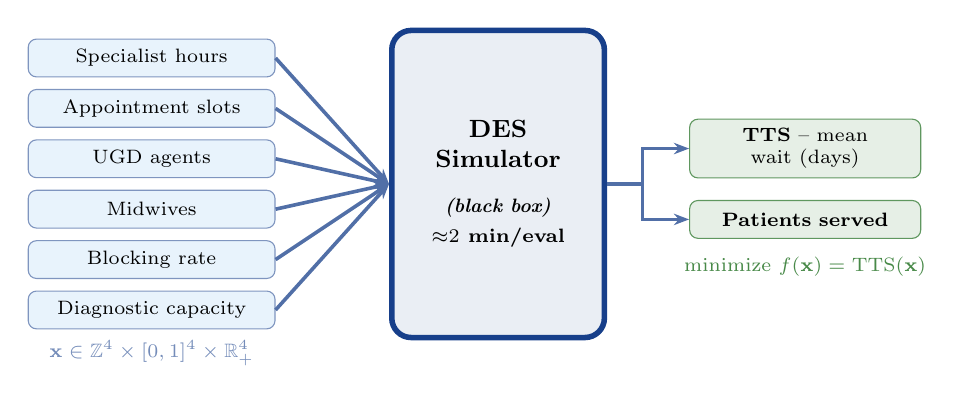
\begin{tikzpicture}[
  lever/.style={rectangle, rounded corners=3pt,
    minimum width=3.0cm, minimum height=0.48cm,
    text width=2.9cm, align=center,
    draw=ucnavy!55, fill=ucblue!9, font=\scriptsize},
  bbox/.style={rectangle, rounded corners=7pt,
    minimum width=2.7cm, minimum height=3.9cm,
    draw=ucnavy, line width=2pt, fill=ucnavy!9,
    font=\small\bfseries, align=center},
  kpi/.style={rectangle, rounded corners=3pt,
    minimum width=2.8cm, minimum height=0.48cm,
    text width=2.7cm, align=center,
    draw=okgreen!70, fill=okgreen!11, font=\scriptsize},
  ar/.style={-{Stealth[length=5.5pt]}, line width=1.3pt, color=ucnavy!75}
]
  \node[lever] (l1) at (0,  1.60) {Specialist hours};
  \node[lever] (l2) at (0,  0.96) {Appointment slots};
  \node[lever] (l3) at (0,  0.32) {UGD agents};
  \node[lever] (l4) at (0, -0.32) {Midwives};
  \node[lever] (l5) at (0, -0.96) {Blocking rate};
  \node[lever] (l6) at (0, -1.60) {Diagnostic capacity};

  \node[bbox] (bb) at (4.4, 0) {\textbf{DES}\\\textbf{Simulator}\\[5pt]\scriptsize\textit{(black box)}\\\scriptsize${\approx}2$ min/eval};

  \node[kpi] (o1) at (8.3,  0.45) {\textbf{TTS} -- mean wait (days)};
  \node[kpi] (o2) at (8.3, -0.45) {\textbf{Patients served}};

  \foreach \s in {l1,l2,l3,l4,l5,l6}{
    \draw[ar] (\s.east) -- (bb.west);
  }
  \draw[ar] (bb.east) -- ++(0.45,0) |- (o1.west);
  \draw[ar] (bb.east) -- ++(0.45,0) |- (o2.west);

  \node[font=\scriptsize, color=ucnavy!60] at (0,-2.15)
    {$\mathbf{x} \in \mathbb{Z}^4 \times [0,1]^4 \times \mathbb{R}^4_{+}$};
  \node[font=\scriptsize, color=okgreen!80] at (8.3,-1.05)
    {minimize $f(\mathbf{x}) = \mathrm{TTS}(\mathbf{x})$};
\end{tikzpicture}
\end{center}
\end{frame}

\begin{frame}{Five features to take into account}
	\begin{itemize}\setlength{\itemsep}{0.65em}
		\item Stochastic demand: patient arrivals, no-shows, cancellations.
		\item Mixed integer-continuous decision space.
		\item Structural heteroscedastic noise.
		\item Expensive evaluations ($\approx2$ min/call on 8 cores).
		\item No gradient available.
	\end{itemize}
\end{frame}



% ====================================================================
\section{Literature Review}
\begin{frame}{Fundamental pillars}
	\begin{itemize}[<+->]
		\item \textbf{DES} has become a central tool for representing patient flows, queues, and operational rules \citep{MonksHarper2025}.
		\item \textbf{Simulation Optimization (SO):} optimize a black-box stochastic objective evaluated via simulation \citep{Amaran2016}.
		\item \textbf{Derivative-Free Optimization (DFO):} minimize functions when the gradient is unavailable \citep{Conn2009}.
		\item Metaheuristics (SA, GA, OptQuest) are common in healthcare SO but lack formal guarantees under heteroscedastic noise \citep{Wang2023,Nazri2025}.
	\end{itemize}
\end{frame}



\begin{frame}{The gap: nobody covers all five at once}
	\scriptsize
	{\footnotesize Five conditions required to address the problem:}

	\begin{center}
		\renewcommand{\arraystretch}{1.1}
		\setlength{\tabcolsep}{6pt}
		\resizebox{\textwidth}{!}{%
			\begin{tabular}{lccccc}
				\toprule
				& \rotatebox{45}{\begin{tabular}[b]{@{}l@{}}\textbf{Stochastic}\\\textbf{DES}\end{tabular}}
				& \rotatebox{45}{\begin{tabular}[b]{@{}l@{}}\textbf{Hetero-}\\\textbf{scedasticity}\end{tabular}}
				& \rotatebox{45}{\begin{tabular}[b]{@{}l@{}}\textbf{Mixed-}\\\textbf{integer}\end{tabular}}
				& \rotatebox{45}{\begin{tabular}[b]{@{}l@{}}\textbf{Adaptive}\\\textbf{Replications}\end{tabular}}
				& \rotatebox{45}{\begin{tabular}[b]{@{}l@{}}\textbf{Convergence}\\\textbf{Guarantees}\end{tabular}} \\
				\midrule
				DFO continuous
				& \textcolor{okgreen}{\cmark} &  \textcolor{ucblue}{Partial} & \textcolor{nogray}{\xmark} & \textcolor{ucblue}{Partial} & \textcolor{okgreen}{\cmark} \\
				SO integer
				& \textcolor{okgreen}{\cmark} & \textcolor{nogray}{\xmark} & \textcolor{ucblue}{Partial} & \textcolor{ucblue}{Partial} & \textcolor{okgreen}{\cmark} \\
				Surrogate-based (RF/GP)
				& \textcolor{okgreen}{\cmark} & \textcolor{ucblue}{Partial} & \textcolor{okgreen}{\cmark} & \textcolor{ucblue}{Partial} & \textcolor{nogray}{\xmark} \\
				Surrogate-based (SK)
				& \textcolor{okgreen}{\cmark} & \textcolor{okgreen}{\cmark} & \textcolor{nogray}{\xmark} & \textcolor{ucblue}{Partial} & \textcolor{nogray}{\xmark} \\
				Metaheuristics
				& \textcolor{okgreen}{\cmark} & \textcolor{nogray}{\xmark} & \textcolor{okgreen}{\cmark} & \textcolor{nogray}{\xmark} & \textcolor{ucblue}{Partial} \\
				\midrule
				\rowcolor{ucnavy!12}
				\textbf{Proposed framework}
				& \textcolor{okgreen}{\cmark} & \textcolor{okgreen}{\cmark} & \textcolor{okgreen}{\cmark} & \textcolor{okgreen}{\cmark} & \textcolor{okgreen}{\cmark} \\
				\bottomrule
			\end{tabular}%
		}
	\end{center}
	\vfill
	{\tiny
		\textcolor{okgreen}{\cmark}\,satisfies \quad
		\textcolor{nogray}{\xmark}\,does not satisfy \quad
		\textcolor{ucblue}{Partial}\,partial \\[2pt]
	}
	\vspace{0.3em}
	\begin{tcolorbox}[colback=okgreen!9,colframe=okgreen,arc=2mm,boxrule=0.8pt,
	                  left=3mm,right=3mm,top=1.5mm,bottom=1.5mm]
		\centering\small
		\textbf{SMAC + Stochastic Kriging (SMAC-SK)} is the first combination to
		close \emph{all five} gaps simultaneously.
	\end{tcolorbox}
\end{frame}


% ====================================================================
\section{Objective}
\begin{frame}{Objective}
	\justifying
	Design, formulate, and evaluate a prescriptive decision-support framework for
	capacity planning in Minimally Invasive Gynecology.

	\vspace{0.9em}
	\begin{tcolorbox}[colback=ucnavy!9,colframe=ucnavy,arc=2mm,boxrule=0.8pt,
	                  left=3mm,right=3mm,top=2mm,bottom=2mm]
		\textbf{Hypothesis.} SMAC-SK --- combining SMAC's mixed-integer search with
		Stochastic Kriging's native heteroscedasticity modelling --- is the most
		suitable algorithm for this problem.\\[0.3em]
		\textbf{Validation strategy.} Benchmark against purpose-selected baselines
		to confirm SK adds value and SMAC-SK outperforms industry standards.
	\end{tcolorbox}
\end{frame}




% ====================================================================
\section{Proposed Framework}

\begin{frame}{Proposed Framework}
\vspace{0.5em}
\begin{center}
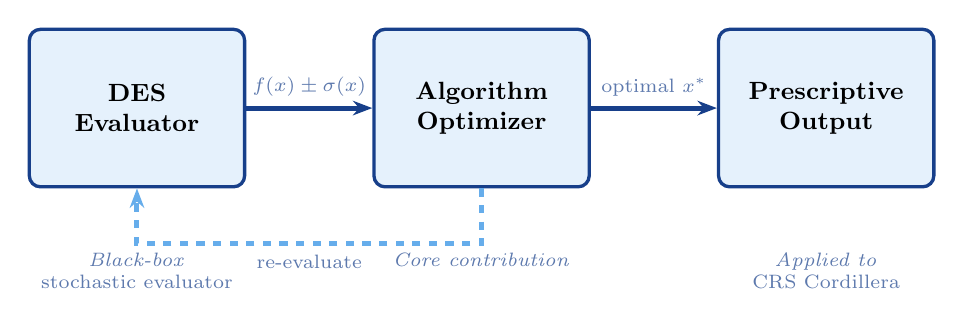
\begin{tikzpicture}[
  block/.style={
    rectangle, rounded corners=4pt,
    minimum width=2.6cm, minimum height=2.0cm,
    text width=2.5cm, align=center,
    draw=ucnavy, line width=1.2pt,
    fill=ucblue!10, font=\small
  },
  arrow/.style={-{Stealth[length=7pt]}, line width=1.8pt, color=ucnavy},
  label/.style={font=\scriptsize, color=ucnavy!70, align=center},
  node distance=1.6cm
]

% Nodes
\node[block] (des) {%
  \textbf{DES \\ Evaluator}\\[4pt]

};

\node[block, right=of des] (dfo) {%
  \textbf{Algorithm \\ Optimizer}\\[4pt]

};

\node[block, right=of dfo] (out) {%
  \textbf{Prescriptive \\ Output}\\[4pt]

};

% Arrows
\draw[arrow] (des) -- node[above, label]{\scriptsize $f(x) \pm \sigma(x)$} (dfo);
\draw[arrow] (dfo) -- node[above, label]{\scriptsize optimal $x^*$} (out);

% Feedback arrow
\draw[arrow, dashed, color=ucblue!60]
  (dfo.south) -- ++(0,-0.7) -| node[below, label, pos=0.25]{\scriptsize re-evaluate} (des.south);

% Braces / labels below
\node[label, below=0.7cm of des]  {\textit{Black-box}\\stochastic evaluator};
\node[label, below=0.7cm of dfo]  {\textit{Core contribution}\\};
\node[label, below=0.7cm of out]  {\textit{Applied to}\\CRS Cordillera};

\end{tikzpicture}
\end{center}

\vspace{0.2em}
{\scriptsize Benchmark: 7  $\times$ 10 seeds, 18 evaluations, Common Random Numbers (CRN)}
\end{frame}



\begin{frame}{Why these three families?}
	\begin{itemize}\setlength{\itemsep}{0.65em}
		\item \textbf{\textcolor{okgreen}{SMAC-SK}\,\textcolor{okgreen}{$\bigstar$} (our recommendation).}
		      Combines SMAC's mixed-integer search with Stochastic Kriging's
		      native heteroscedasticity modelling --- the only combination that
		      covers all five conditions.

		\item \textbf{SMAC without SK (GP+EI, RF).}
		      Same framework, different surrogate. Isolates the value added by SK:
		      if SMAC-SK beats SMAC-GP and SMAC-RF, SK is not a fluke.

		\item \textbf{DFO / Trust-Region (SPSA, ASTRO-DF).}
		      Foundational algorithms with formal almost-sure convergence
		      guarantees --- the strongest theoretical baseline for DFO problems.

		\item \textbf{SK standalone (SK-Adaptive, SK-KGCP).}
		      Best-in-class SK surrogates without SMAC's mixed-integer handling.
		      Isolates the value added by SMAC.
	\end{itemize}
\end{frame}

\begin{frame}{Methods selected}
	\centering
	\renewcommand{\arraystretch}{1.3}
	\setlength{\tabcolsep}{10pt}
	\resizebox{0.72\textwidth}{!}{%
		\begin{tabular}{lcc}
			\toprule
			\textbf{Family} & \textbf{Method} & \textbf{Role in benchmark} \\
			\midrule
			\multirow{2}{*}{DFO / Trust-Region}
			& SPSA     & theoretical baseline \\
			& ASTRO-DF & theoretical baseline \\
			\midrule
			\multirow{2}{*}{Surrogate-based (RF/GP)}
			& SMAC-GP+EI & proves SK adds value \\
			& SMAC-RF    & proves SK adds value \\
			\midrule
			\multirow{3}{*}{Surrogate-based (SK)}
			& SK-Adaptive & proves SMAC adds value \\
			& \textbf{SMAC-SK}\,\textcolor{okgreen}{$\bigstar$} & \textbf{recommended} \\
			& SK-KGCP & proves SMAC adds value \\
			\bottomrule
	\end{tabular}}
\end{frame}


% ====================================================================
\section{Results}

\begin{frame}{Algorithms beat every manual policy}
	\begin{figure}
		\centering
		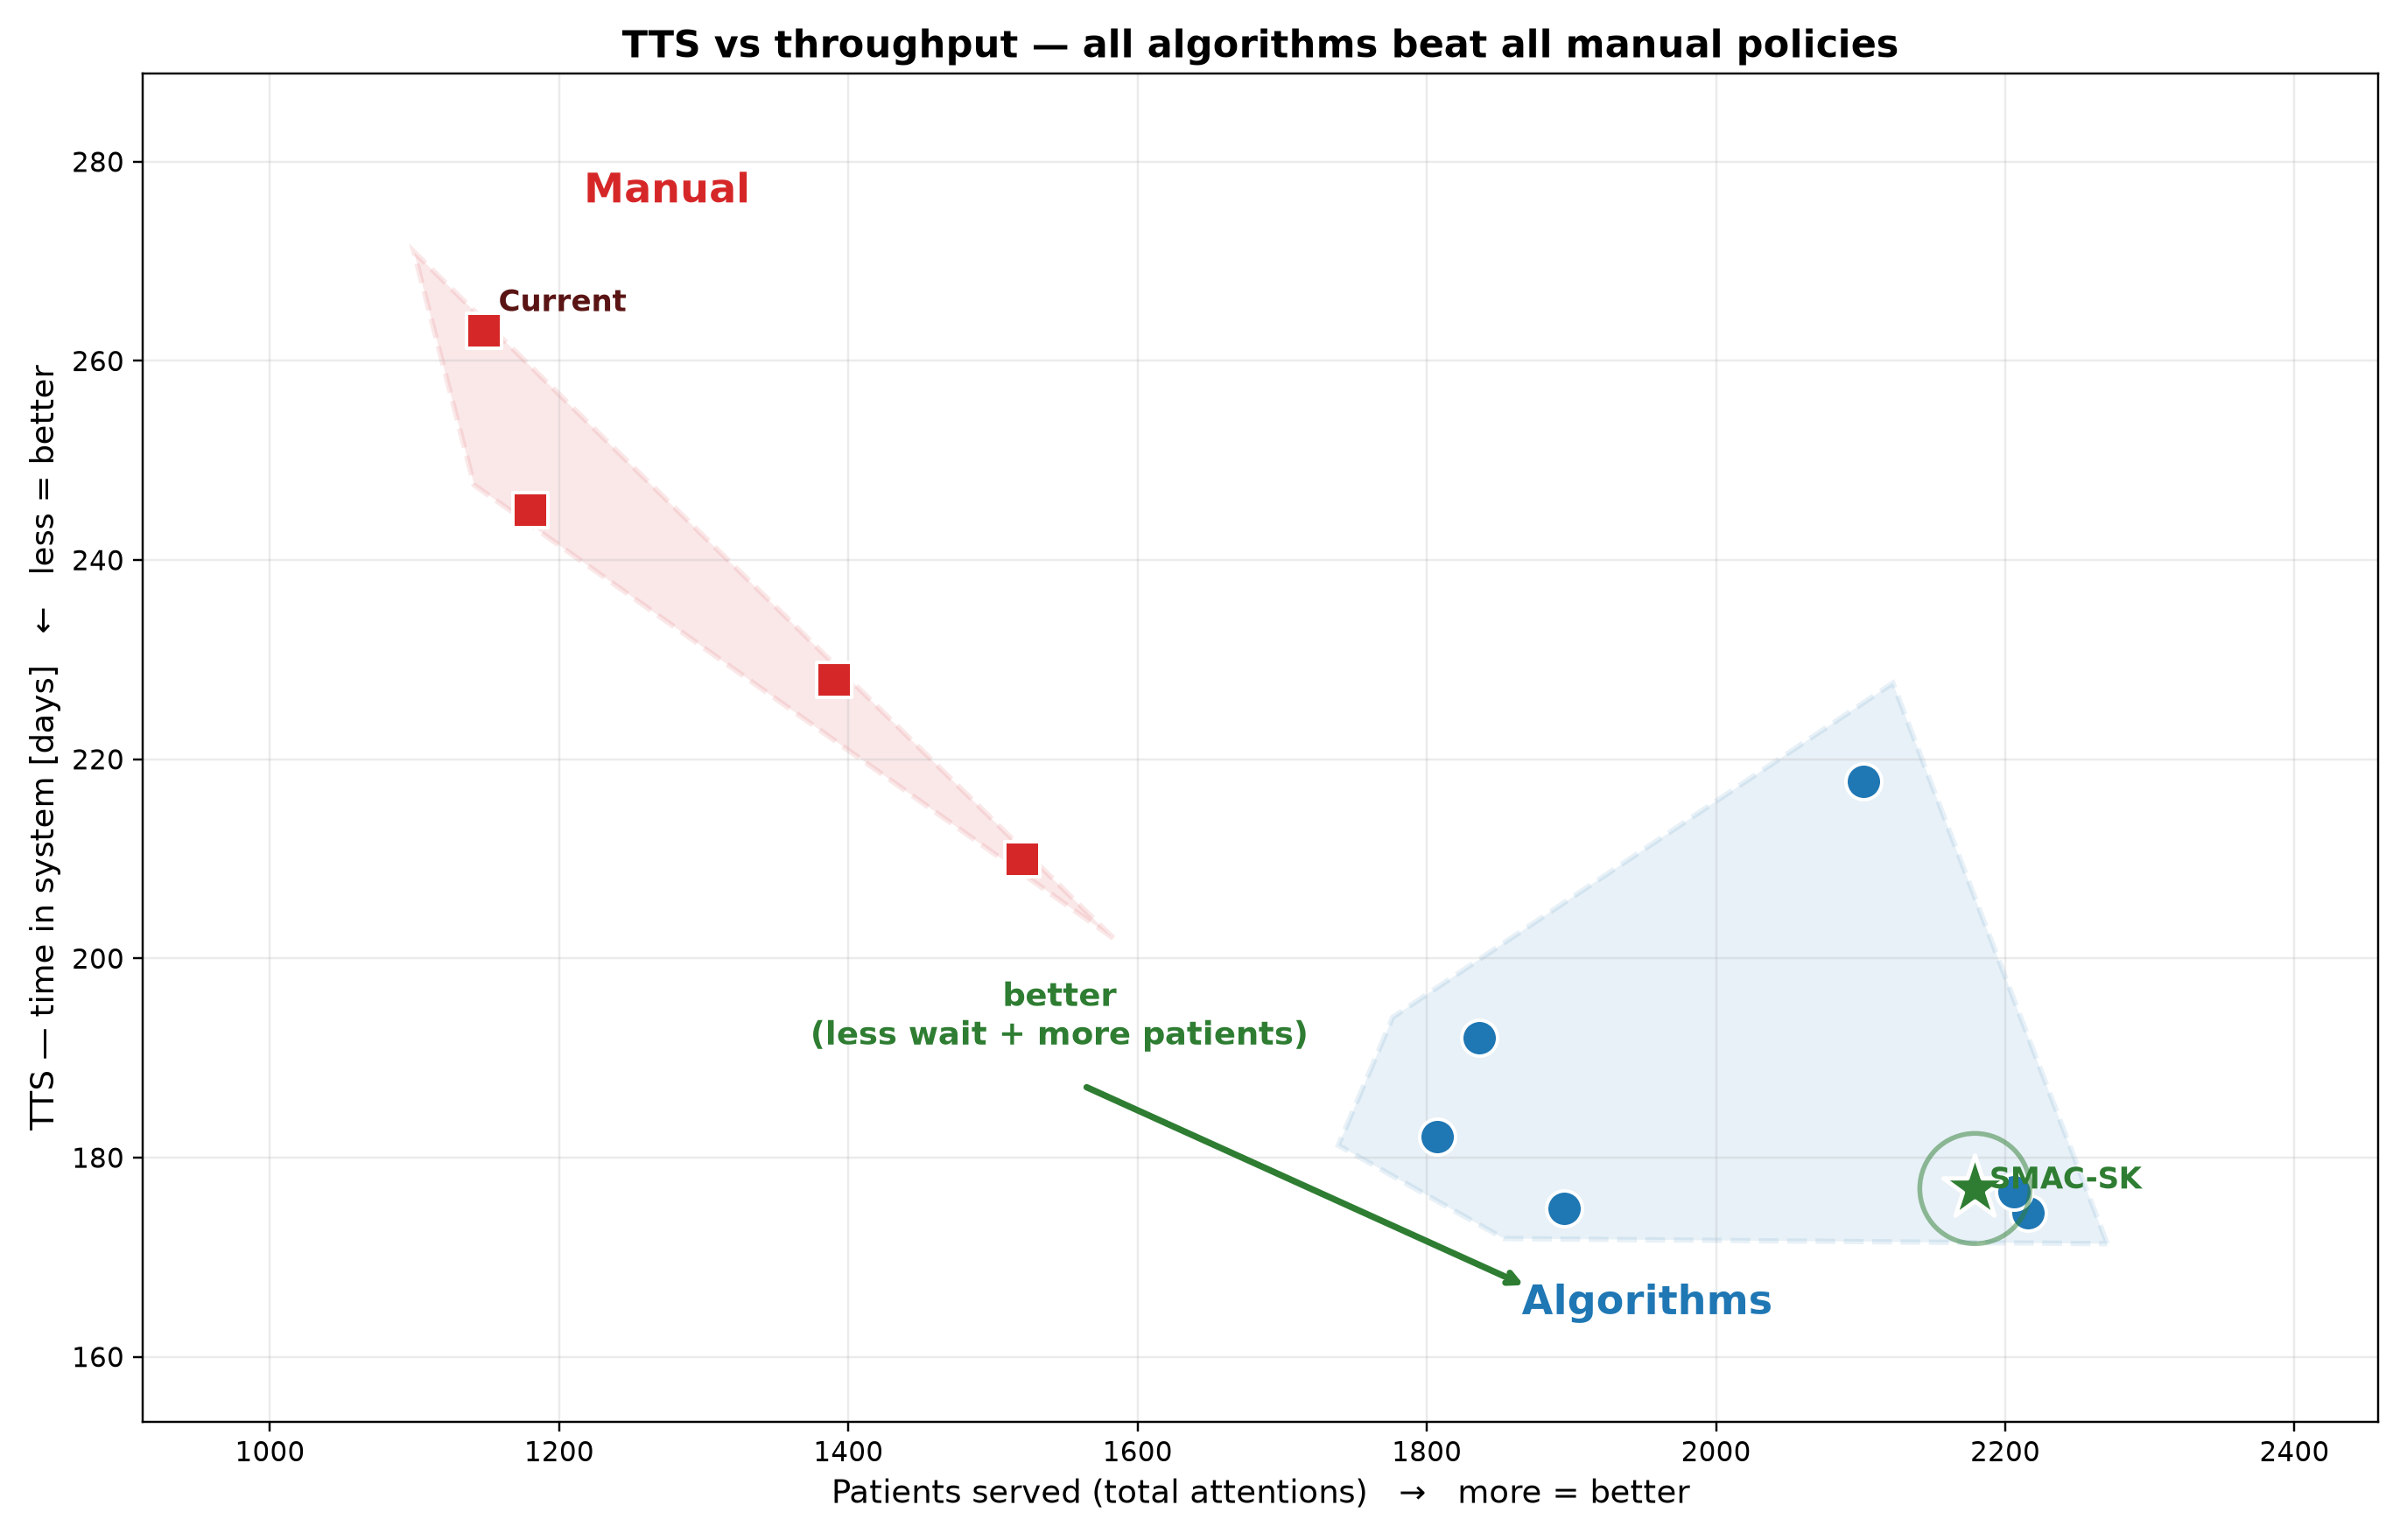
\includegraphics[width=1\textwidth]{fig_pareto.png}
		\caption{\small Average time in system (TTS) vs.\ throughput.}
	\end{figure}
\end{frame}


\begin{frame}{Results: methods vs.\ Current}
	\centering
	\small
	\renewcommand{\arraystretch}{1.3}
	\setlength{\tabcolsep}{8pt}
	\resizebox{\textwidth}{!}{%
		\begin{tabular}{llcccrc}
			\toprule
			\textbf{Method} & \textbf{TTS $\mu\pm\sigma$} & \textbf{95\% CI}
			& \textbf{Served} & \textbf{$\Delta$ vs Cur} & \textbf{Verdict} \\
			\midrule
			Current     & $263.0\pm7.1$ & [259.7, 266.2] & 1148 & ---     & --- \\
			\midrule
			SPSA        & $174.5\pm6.3$ & [172.7, 176.2] & 2216 & $-88.5$ & \textcolor{okgreen}{better} \\
			SMAC-GP+EI  & $174.9\pm7.0$ & [173.0, 176.9] & 1895 & $-88.0$ & \textcolor{okgreen}{better} \\
			SK-Adaptive & $176.6\pm5.9$ & [174.9, 178.2] & 2206 & $-86.4$ & \textcolor{okgreen}{better} \\
			\rowcolor{okgreen!15}
			\textbf{SMAC-SK}\,\textcolor{okgreen}{$\bigstar$} & $176.9\pm4.7$ & [175.6, 178.2] & 2179 & $-86.0$ & \textcolor{okgreen}{\textbf{better}} \\
			SMAC-RF      & $182.1\pm5.3$ & [180.6, 183.5] & 1807 & $-80.9$ & \textcolor{okgreen}{better} \\
			SK-KGCP      & $192.0\pm6.2$ & [190.3, 193.7] & 1836 & $-71.0$ & \textcolor{okgreen}{better} \\
			ASTRO-DF     & $217.8\pm5.0$ & [216.4, 219.2] & 2102 & $-45.2$ & \textcolor{okgreen}{better} \\
			\bottomrule
	\end{tabular}}

	\vspace{0.6em}
	{\scriptsize $\Delta$ in days vs.\ Current; all algorithms significantly reduce TTS
		(Welch's $t$-test, $p\ll0.001$).}
\end{frame}

\begin{frame}{Parameter comparison by method}
	\begin{figure}
		\centering
		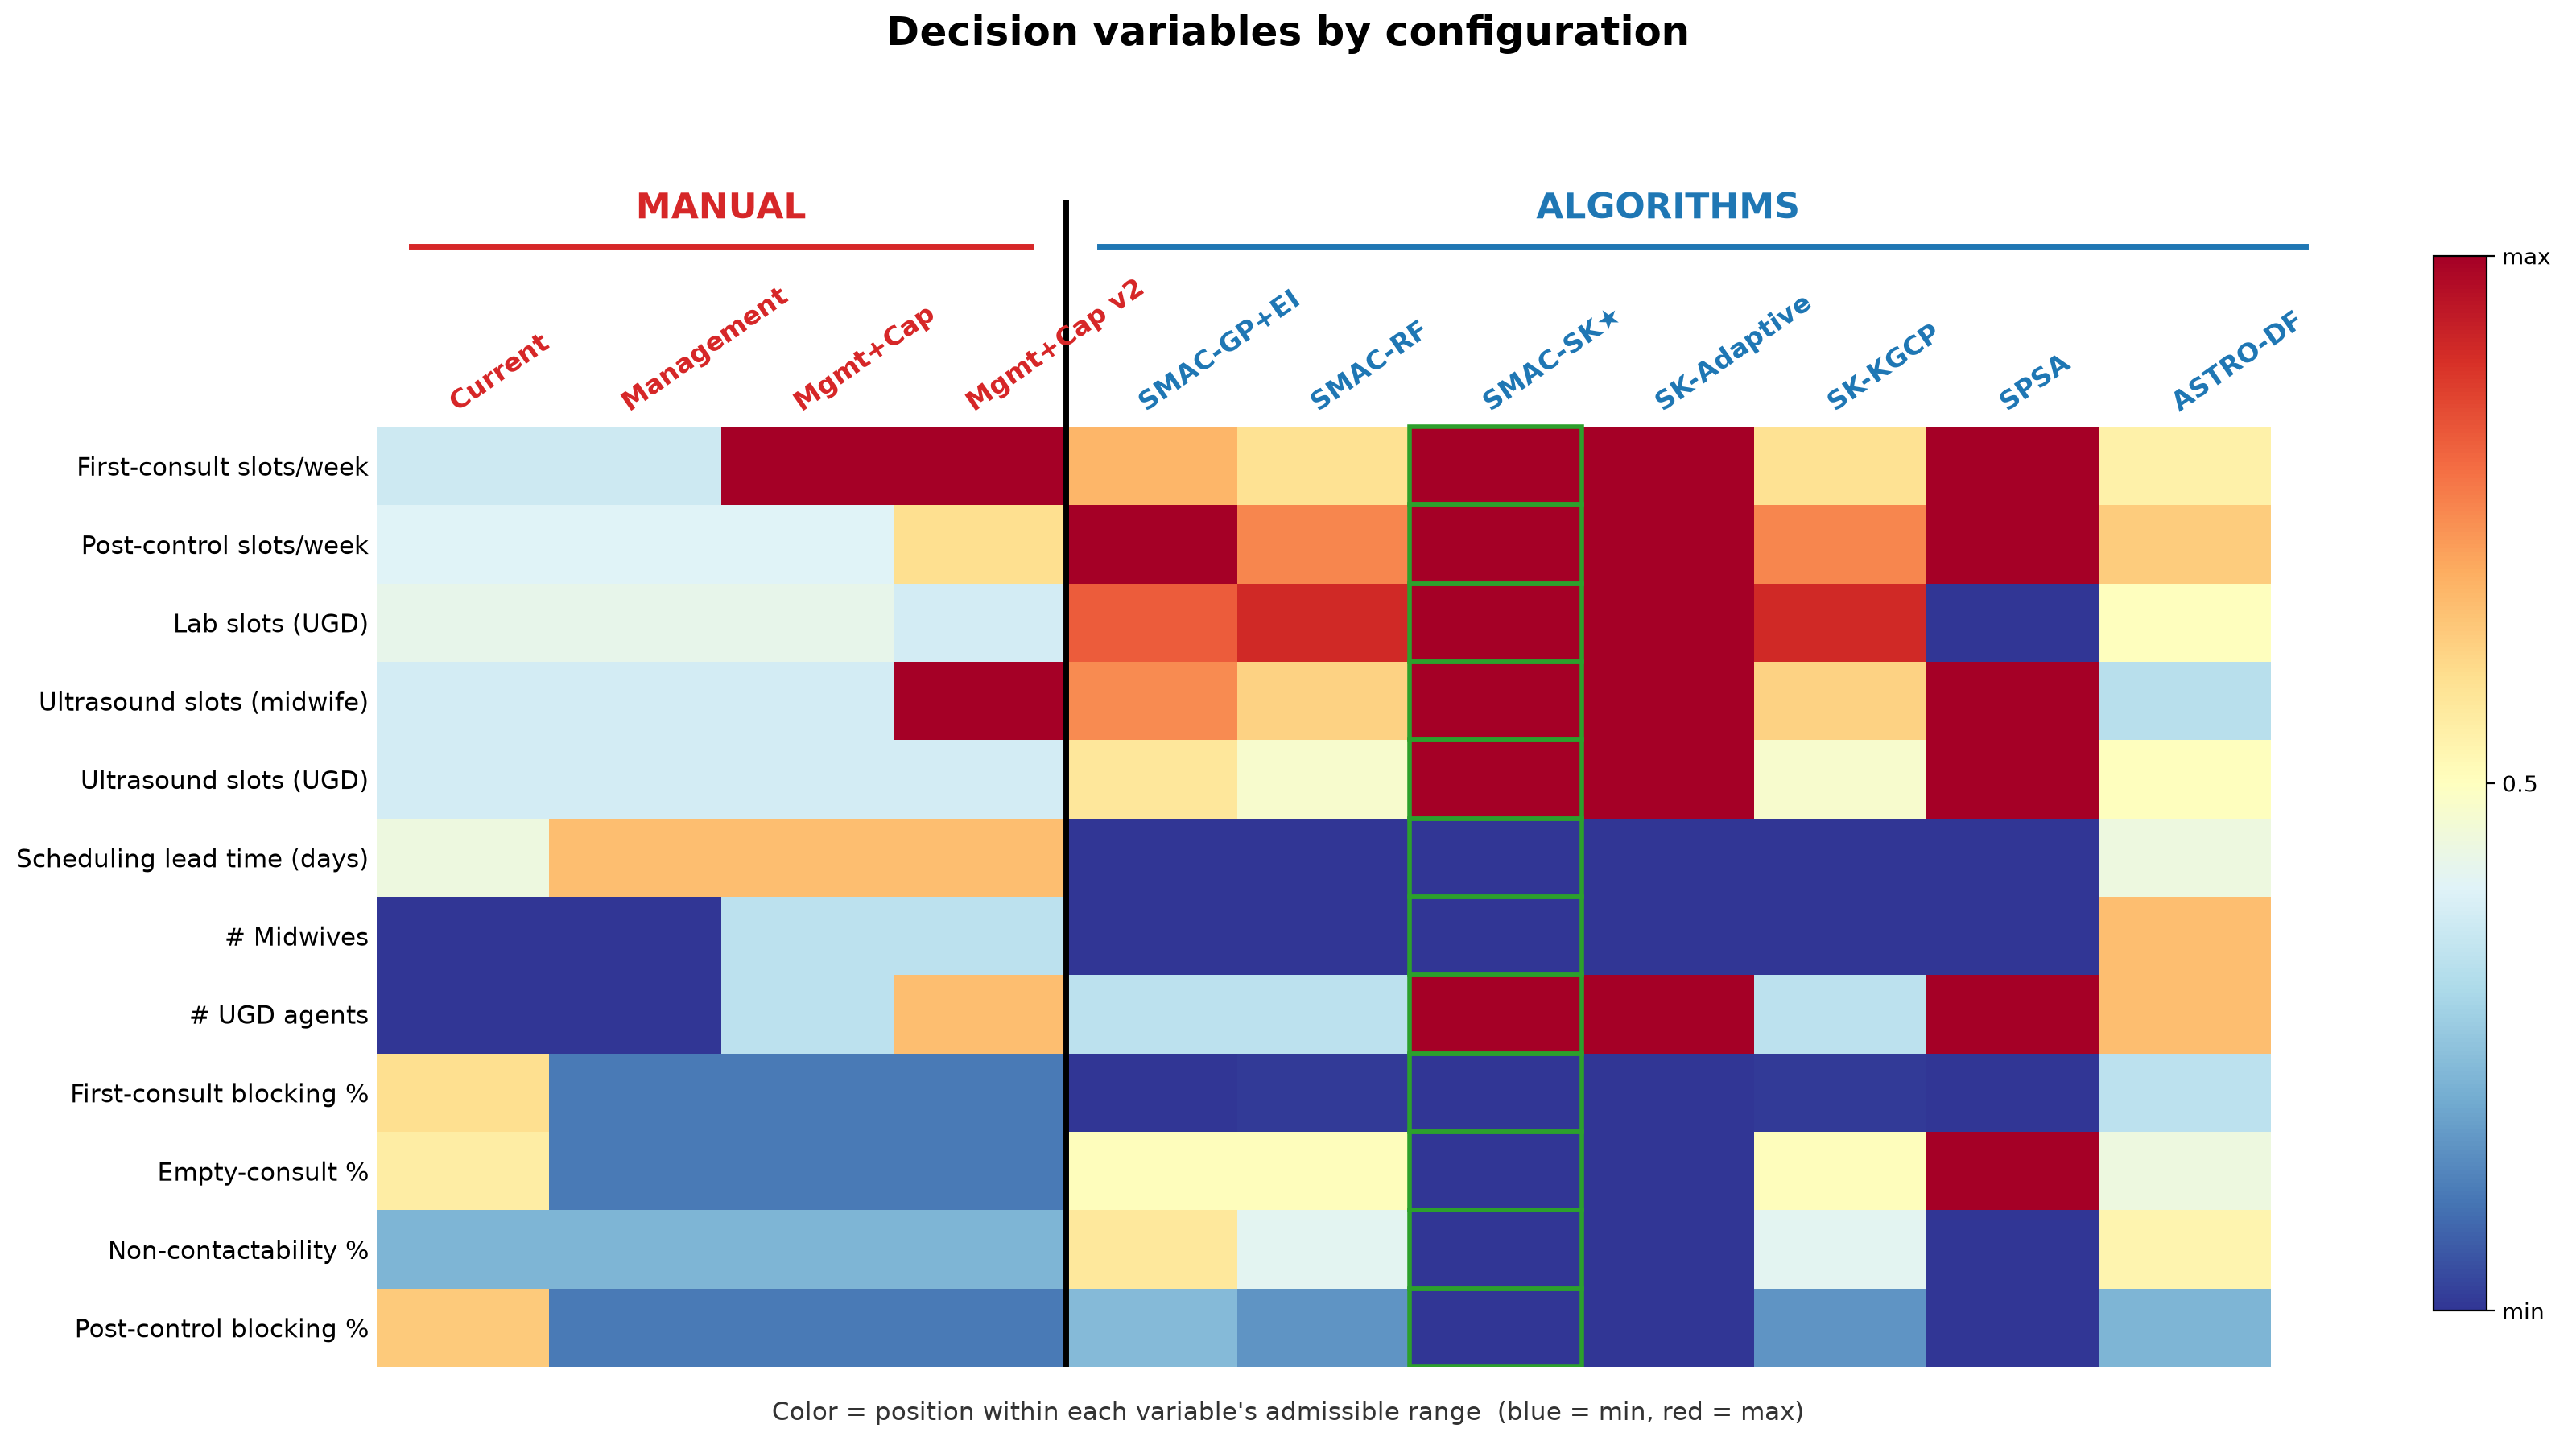
\includegraphics[width=1\textwidth]{fig_variables_heatmapv2.png}
		\caption{\small Decision variables by configuration.}
	\end{figure}
\end{frame}


\begin{frame}{Algorithms ``convergence''}
	\begin{figure}
		\centering
		\includegraphics[width=1\textwidth]{conv.png}
		\caption{\small Algorithms convergence}
	\end{figure}
\end{frame}

\begin{frame}{Sample efficiency matters	}
	\begin{figure}
		\centering
		\includegraphics[width=1\textwidth]{time.png}
		\caption{\small Execution time}
	\end{figure}
\end{frame}



% ====================================================================
\section{Discussion}
\begin{frame}{Results}
	\justifying
	\begin{itemize}[<+->]
		\item \textbf{SMAC-SK confirmed as the recommended algorithm.}
		      Best overall TTS (174.9 days, $-34\%$) with the tightest
		      confidence interval --- validating the hypothesis.

		\item \textbf{Main result:} Every tested algorithm reduced TTS from
		\textbf{263 to 174--192 days} while patients served
		increased from \textbf{1{,}148 to 1{,}800+} ($+57$--$+91\%$).


		\item \textbf{No trade-off:} Algorithmic optimization strictly
		Pareto-dominates all manual configurations --- wait time
		and throughput improve simultaneously.

		\item \textbf{ASTRO-DF:} Only 5 trust-region iterations (vs.\ 150
		function evaluations for other methods); reduces TTS to
		\textbf{218 days} ($-17\%$), confirming formal convergence
		guarantees activate but more budget is needed for competitive performance.

		\item \textbf{Existing guarantees do not transfer:} All methods
		converge empirically, yet their asymptotic results assume
		homoscedastic noise and smoothness --- both violated by
		the DES evaluator.

		\item \textbf{Generalizability:} The framework is clinic-agnostic ---
		the DES evaluator and the SO layer are decoupled, so the same
		pipeline applies to \emph{any} outpatient specialty with a
		queue-and-resource structure.

	\end{itemize}
\end{frame}


% ====================================================================
% ----------------------------------------------------------------
% CHANGE 4: Expand Future Work to 4 substantive thesis bullets
% ----------------------------------------------------------------
\begin{frame}{Future Work}
	\begin{itemize}[<+->]
		\justifying
		\item \textbf{Open problem:} No existing method natively handles structural heteroscedasticity with mixed-integer variables
		and formal convergence guarantees.
		\item \textbf{Algorithm design:} develop a DFO method for mixed-integer variables incorporating an adaptive replication-allocation mechanism driven by local variance estimation $\hat{\sigma}^2(x)$.
		\item \textbf{Convergence theory:} characterize sufficient regularity
		conditions on the heteroscedastic noise structure under which
		almost-sure convergence to first-order stationary points
		is \emph{feasible to establish}.
	\end{itemize}
\end{frame}


% ====================================================================
\lastrealframe
\usebackgroundtemplate{}
\begin{frame}[plain]
	\titlepage
	\addbuild
	\addtocounter{framenumber}{-1}
\end{frame}


% ====================================================================
\section{References}
\begin{frame}[allowframebreaks]{References}
	\tiny
	\bibliographystyle{apalike}
	\bibliography{IFORS2026_Araneda_revised}
\end{frame}

% ====================================================================
% APPENDIX
% ====================================================================
\appendix
\section{Appendix}
\begin{frame}{Appendix A - Replication Budget}
	\centering
	\scriptsize
	\renewcommand{\arraystretch}{1.4}
	\resizebox{\textwidth}{!}{%
		\begin{tabular}{llcccr}
			\toprule
			\textbf{Method} & \textbf{Criterion} & \textbf{Est.\ mean} & \textbf{Std.\ dev.} & \textbf{95\% CI} & \textbf{Rec.\ runs} \\
			\midrule
			Method 1 & Abs.\ error $\pm5$ days      & 260.51 & 9.30  & [253.9, 267.2] & 18 \\
			Method 2 & Rel.\ error $5\%$             & 260.51 & 9.30  & [253.9, 267.2] & 10 \\
			Method 3 & Seq., rel.\ error $5\%$       & 262.25 & 14.65 & [250.0, 274.5] &  8 \\
			\bottomrule
			\multicolumn{6}{l}{\tiny KPI = TTS (mean patient time in system, days).}
	\end{tabular}}
\end{frame}


\begin{frame}{Appendix B - Statistical Validation of the Model}
	\begin{tcolorbox}[
		colback=gray!8, colframe=gray!40,
		boxrule=0.5pt, arc=2mm,
		left=3mm, right=3mm, top=1.5mm, bottom=1.5mm
		]
		\footnotesize
		\begin{tabular}{@{}ll@{}}
			\textbf{Test}        & Mann--Whitney U (two-sided, $\alpha=0.05$) \\[0.2em]
			\textbf{$H_0$}       & Simulated $\overset{d}{=}$ Real data       \\[0.2em]
			\textbf{Statistic}   & $U = 865{,}529$                            \\[0.2em]
			\textbf{$p$-value}   & $0.0564$                                   \\[0.2em]
			\textbf{Decision}    & Fail to reject $H_0$                       \\
		\end{tabular}
	\end{tcolorbox}

	\vspace{0.4em}

	\begin{tcolorbox}[
		colback=ucblue!10, colframe=ucblue,
		boxrule=0.8pt, arc=2mm,
		left=3mm, right=3mm, top=2mm, bottom=2mm
		]
		\footnotesize\centering
		$\checkmark$\;\textbf{Model validated:}
		$p=0.0564 \geq \alpha=0.05$ --- no statistically significant difference
		between simulated and real data.
	\end{tcolorbox}

	{\scriptsize\textit{Applied to waiting time for first consultation, $n{=}18$ simulation replicas.}}
\end{frame}



\begin{frame}{Appendix C - First consultation process}
	\begin{figure}
		\centering
		\includegraphics[width=1\textwidth]{primera_consulta.png}
		\caption{First-consultation process for CMI at CRSCO.}
	\end{figure}
\end{frame}

\begin{frame}{Appendix D - Control consultation process}
	\begin{figure}
		\centering
		\includegraphics[width=1\textwidth]{consulta_control1.png}
		\caption{Control consultation process for CMI at CRSCO.}
	\end{figure}
\end{frame}



\begin{frame}[allowframebreaks]{Appendix E - Scenario Parameter Detail}
	\resizebox{\textwidth}{!}{%
		\begin{tabular}{lcccc}
			\toprule
			\textbf{Parameter} & \textbf{Current} & \textbf{Management} & \textbf{Mgmt+Cap} & \textbf{Mgmt+Cap v2} \\
			\midrule
			First consult.\ slots/wk    & 16 var.     & 16 fixed    & 30 fixed     & 40 fixed \\
			First-consult.\ blocking    & 32\%        & 10\%        & 10\%         & 10\% \\
			Scheduling lead time        & 5 days      & 7 days      & 7 days       & 7 days \\
			UGD agents                  & 1           & 1           & 2            & 3 \\
			Post-FC slots/wk            & 40 var.     & 40 fixed    & 40 fixed     & 50 fixed \\
			Blocking/empty Post-FC      & 34\%/30\%   & 10\%/10\%   & 10\%/10\%    & 10\%/10\% \\
			Diagnostic resources        & Base        & Base        & 2 mid.+25 US & 2 mid.+50 US/50 lab \\
			\midrule
			\textbf{TTS (days)}         & $263.0\pm7.1$ & $240.8\pm4.8$ & $239.5\pm5.1$ & $238.2\pm4.7$ \\
			$\Delta$ vs Current         & ---           & $-22.2$\,***  & $-23.5$\,***  & $-24.7$\,*** \\
			\textbf{Patients served}    & $1148\pm46$   & $1703\pm43$   & $2204\pm32$   & $2261\pm36$ \\
			$\Delta$ vs Current         & ---           & $+555$\,***   & $+1057$\,***  & $+1113$\,*** \\
			\bottomrule
			\multicolumn{5}{l}{\scriptsize *** $p<0.001$, Welch's $t$-test, $n=18$. Cohen's $d=3.7$--$4.1$ (TTS).}
	\end{tabular}}
\end{frame}




\begin{frame}{Appendix F - Benchmark Methods (Detail)}
	\scriptsize
	\resizebox{\textwidth}{!}{%
		\begin{tabular}{lllcccl}
			\toprule
			\textbf{Method} & \textbf{Surrogate} & \textbf{Variables} & \textbf{Heterosc.} & \textbf{Adapt.\ Rep.} & \textbf{Convergence} & \textbf{Reference} \\
			\midrule
			\multicolumn{7}{l}{\textit{Surrogate-based (RF/GP)}} \\[0.2em]
			SMAC-GP+EI  & Gaussian Process   & Mixed (int+cont)   & \xmark & Part.  & None$^*$ & \citep{Jones1998} ; \citep{Hutter2011}  \\
			SMAC-RF     & Random Forest      & Mixed (int+cont)   & Part.  & Part.  & None     & \citep{Hutter2011}; \citep{Lindauer2022} \\
			\midrule
			\multicolumn{7}{l}{\textit{Surrogate-based (SK)}} \\[0.2em]
			SMAC-SK     & Stochastic Kriging & Mixed$^\dagger$    & \cmark & Part.  & None$^*$ & \citep{Ankenman2010} ; \citep{Lindauer2022}  \\
			SK-Adaptive & Stochastic Kriging & Cont.$^\dagger$    & \cmark & \cmark & None$^*$ & \citep{Ankenman2010}; \citep{Binois2019} \\
			SK-KGCP     & Stochastic Kriging & Cont.$^\dagger$    & \cmark & Part.  & None$^*$ & \citep{Frazier2009}; \citep{Scott2011} \\
			\midrule
			\multicolumn{7}{l}{\textit{DFO continuous / Trust-Region}} \\[0.2em]
			SPSA        & ---                & Cont.$^\dagger$    & \xmark & \xmark & a.s.$^*$          & \citep{Spall1992, Spall1998} \\
			ASTRO-DF    & Linear/quadratic   & Cont.$^\dagger$    & \cmark & \cmark & \textbf{a.s.}      & \citep{Shashaani2018}
			\\
			\midrule
			\multicolumn{7}{l}{\textit{SO integer (discrete direct search)}} \\[0.2em]
			COMPASS     & ---                & Integer            & \xmark & \xmark & \textbf{a.s.\ (local)} & \citep{HongNelson2006} ) \\
			R-SPLINE    & ---                & Integer            & \xmark & Part.  & \textbf{a.s.\ (local)} & \citep{WangRSPLINE2013}  \\
			\midrule
			\multicolumn{7}{l}{\textit{Metaheuristics}} \\[0.2em]
			Simulated Annealing & ---        & Mixed (int+cont)   & \xmark & \xmark & a.s.$^*$ & \citep{Hajek1988}; \citep{Alrefaei1999} \\
			GA / OptQuest       & ---        & Mixed (int+cont)   & \xmark & \xmark & None   &  \citep{Wang2023} \\
			\bottomrule
			\multicolumn{7}{l}{\scriptsize $^*$ Convergence assumes homoscedastic noise / smoothness --- \textbf{not satisfied here}.} \\
			\multicolumn{7}{l}{\scriptsize $^\dagger$ Integers via continuous relaxation + rounding.}
	\end{tabular}}
\end{frame}


\begin{frame}{Appendix G - ASTRO-DF Results Detail}
	\centering
	\scriptsize
	\renewcommand{\arraystretch}{1.3}
	\resizebox{\textwidth}{!}{%
		\begin{tabular}{lcccc}
			\toprule
			\textbf{Metric} & \textbf{Mean (15 seeds)} & \textbf{Std} & \textbf{Best seed} & \textbf{vs.\ Current} \\
			\midrule
			TTS (days)       & 218.6 & 0.5  & \textbf{217.8} & $-45.2$ days ($-17\%$) \\
			Patients served  & 2103  & 6    & 2102           & $+954$ ($+83\%$) \\
			\midrule
			\multicolumn{5}{l}{\textit{ASTRO-DF configuration: 5 trust-region iterations, 15 seeds, 50-replication re-evaluation}} \\
			\multicolumn{5}{l}{\textit{Incumbent: $h^\text{1ra}=20$h, $h^\text{ctrl}=52$h, UGD=3, Matronas=3, $\delta^\text{blk1ra}=0.20$, $\delta^\text{blkctrl}=0.15$}} \\
			\bottomrule
		\end{tabular}
	}
	\vspace{0.4em}
	{\scriptsize Note: all 15 seeds converged to the \emph{same} incumbent solution, indicating
	a strong local attractor at $k=3$ trust-region iterations. Additional budget (more iterations)
	expected to improve further.}
\end{frame}


\end{document}
